\chapter{Elliptic Curves}
%references http://infosec.pusan.ac.kr/wp-content/uploads/2019/09/Pairings-For-Beginners.pdf
Generally speaking, elliptic curves are "curves" defined in geometric planes like the Euklidean or the projective plane over some given field. One of the key features of elliptic curves over finite fields from the point of view of cryptography is their set of points has a group law, such that the resulting group is finite and cyclic and it is believed that the discrete logarithm problem on these groups is hard. 

A special class of elliptic curves are so called \textit{pairing friendly curve}, which have a notation of pairing as defined in XXX, that has cryptographicall nice prperties. Those curve are useful in the development of SNAKS, since they allow to compute so called R1CS-satisfiability "in the exponent" (THIS HAS TO BE REWRITTEN WITH WAY MORE DETAIL)

In this chapter we introduce epileptic curves as they are used in pairing based approaches to the construction of snarks. 

The eliptic curves we consider are all defined over prime fields or prime field extensions and the reader should be familiar with the contend of the previous section on those fields.

In its most generality elliptic curves are defined as a smooth projective curve of genus 1 defined over some field $\F$ with a distinguished $\F$-rational point, but this definition is not very useful for the introductary character of this book. We will therefore look at $3$ more practical definitions in the following sections, by introducing Weierstraß, Montgommery and Edwards curves. All of them are useful in cryptography and nesessary to understand for the contnuation of the book.

\section{Elliptic Curve Arithmetics}

\subsection{Short Weierstraß Curves}
In this section we introduce the so called short Weierstraß curves, which are the most general types of curves over finite fields of characteristic greater then $3$. 

We start with their reprrsention in affine space. This reprresentation has the advantage that affine points are just pairs of numbers which is more convinient to work with for the beginner. However it has the disadvantage that a special "point at infinity" that is not a point on the curve, is necessary to describe the group structure. We introduce the elliptic curve group law and describe elliptic curve scalar multiplication, which is nothing but an instatation of the exponential map from general cyclic groups.

Then we look at the projective representation of short Weierstrass curves. It has the advantage that no special sybol is necessary to represent the point at infinity but comew with the drawback that projective points are classes of numbers, which might be a bit unusual for a beginner.

We finish this section with an explicit equivalence that transforms affine representations into projective once and vice versa.

\paragraph{Affine short Weierstraß form} Probably the least abstract and most straight forward way to introduce elliptic curves for beginners is the so called affine representation of a short Weierstraß curve. To see what this is, let $\F_q$ be a finite field of characteristic $char(\F)> 3$ and $a,b\in \F_q$ two field elements such that $\Zmod{6\cdot(4a^3+ 27b^2)}{q}\neq 0$. Then a \textbf{short Weierstrass elliptic curve} $E(\F_q)$ over $\F_q$ in its affine representation is the set
\begin{equation}
\label{def_short_weierstrass_curve}
E(\F_q) = \{(x,y)\in \F_q\times \F_q\;|\; y^2=x^3+ax+b \} \bigcup \{\Oinf\}
\end{equation}
of all pairs of field elements $(x,y)\in \F_q\times \F_q$, that satisfy the short Weierstrass cubic equation $y^2=x^3+ax+b$, together with a distingushid symbol $\Oinf$, called the \textbf{point at infinity}.

To brake this complicated looking definition down into simple terms, a short Weierstraß elliptic curve is nothing but the set of all pairs of $x$ and $y$ coordinates, that satisfy the equation $y^2 = x^3 + a\cdot x +b$ together with a special symbol. 

The term "curve" appears, because in the ordinary 2 dimensional plane $\R^2$,
the set of all points $(x,y)$ that satisfy $y^2 = x^3 +ax +b$ looks like a curve. We should note however, that visualizing elliptic curves over finite fields as "curves" has its limitations and we will therefore not stress the geometric picture too much, but focus on the compuational properties instead.

The identity $\Zmod{6\cdot(4a^3+ 27b^2)}{q}\neq 0$ ensures that the curve is  non-singular, which means that the curve has no cusps or self-intersections.

\begin{notation}
In the literature, the set $E(\F_q)$, which includs the sybol $\mathcal{O}$ is often called the set of \textit{rational points} of the elliptic curve, in which case the curve itself is usually written as $E/\F_q$. However in what follows we will frequently identify an elliptic curve with its set of rational points and therefore use the symbol $E(\F_q)$ instead. This is possible in our case, since we only really care about the group structure of the curve in consideration.
\end{notation}
When dealing with elliptic curves compuations can quickly become cumbersome and tedious. So on the one hand side the reader is adviced to do as many compuations in a pen and paper style as possible. This helps a lot to get a deeper understanding for the details. On the other hand side however, compuations are sometimes simply to large to be done by hand and one might get lost in the details. Fortunately sage is very helpful in dealing with elliptic curves. One we to define elliptic curves and work is them goes like this:
\begin{sagecommandline}
sage: F5 = GF(5) # define the base field
sage: a = F5(2) # parameter a
sage: b = F5(4) # parameter b
sage: F5(6)*(F5(4)*F5(2)^3+F5(27)*F5(4)^2) != F5(0)
sage: # short Weierstrass curve 
sage: E = EllipticCurve(F5,[a,b]) # y^2 == x^3 + ax +b 
sage: P = E(0,2) # 2^2 == 0^3 + 2*0 + 4
sage: P.xy() # affine coordinates
sage: INF = E(0) # point at infinity
sage: try: 	# point at infinity has no affine coordinates
....:     INF.xy()
....: except ZeroDivisionError:
....:     pass

\end{sagecommandline}
The following three examples will give a more practical understanding of what an elliptic curve is and how we can compute them. The reader is adviced to read them carefully and ideally to parallel the computation themselfs. We will repeatedly build on these example in this chapter and use the second example at various places in this book.
\begin{example}Consider the prime field $\F_5$ from example (XXX). If we choose $a=1$ and $b=1$ then $\kongru{4a^3+ 27b^2}{1}{5}$ and the corresponding elliptic curve $E_1(\F_5)$ is given by all pairs $(x,y)$ from $\F_5$ such that $y^2=x^3+x+1$. 

For example if we choose $(x,y)=(1,1)$, we see that $1^2 \neq 1^3+1 + 1$ and hence the pair $(1,1)$ is not an element of the curve $E_1(\F_5)$. On the other hand $(x,y)=(2,1)$ gives $1^2 = 2^3 + 2 + 1$ and hence the pair $(2,1)$ is an element of $E_1(\F_5)$. Doing the same computations for all 25 combinations of pairs in $\F_5$, gives the set of rational points as 
$$
E_1(\F_5) = \{\Oinf, (0,1),(2,1),(3,1),(4,2),(4,3),(0,4),(2,4),(3,4)\}
$$
So our elliptic curve is a set of $9$ elements. $8$ of which are pairs of numbers and one special symbol $\Oinf.$ We can also invoke sage to compute this elliptic curve. 
\begin{sagecommandline}
sage: F5 = GF(5)
sage: E1 = EllipticCurve(F5,[1,1])
sage: try: # valid point
....:     E1(2,1).xy() # 1^2 == 2^3 + 2 + 1
....: except TypeError:
....:     pass
sage: try: # invalid point
....:     E1(1,1).xy() # 1^2 != 1^3 + 1 + 1
....: except TypeError:
....:     pass
\end{sagecommandline}
% sage: AffinePoints = [P.xy() for P in E1.points() if P.order > 1]
\end{example}
\begin{example}[Moon-JubJub] Consider the prime field $\F_{13}$. If we choose $a=8$ and $b=8$ then $\kongru{4a^3+ 27b^2}{6}{13}$ and the corresponding elliptic curve $MJJ(\F_{13})$ is given by all pairs $(x,y)$ from $\F_13$ such that $y^2=x^3+8x+8$ holds. Since there are $169$ pairs of elements from $\F_{13}$, computing the set of curve points is a bit to much work and we invoke sage instead. We get
\begin{sagecommandline}
sage: F13 = GF(13)
sage: MJJ = EllipticCurve(F13,[8,8])
sage: AffinePoints = [P.xy() for P in MJJ.points() if P.order() > 1]
\end{sagecommandline}
\begin{multline*}
MJJ(\F_{13}) = \{\Oinf, (1, 2), (1, 11), (4, 0), (5, 2), (5, 11), (6, 5), (6, 8), (7,2), (7, 11), \\ (8, 5), (8, 8), (9, 4), (9, 9), (10, 3), (10,
10), (11, 6), (11, 7), (12, 5), (12, 8)\}
\end{multline*}
We call $MJJ(\F_{13})$ the \textit{Moon-JubJub} curve. As we will see in what follows this curve is kind of special as it is possible to represent it in two alternitive forms, called a Montgomery and a twisted Edwards form (See xxx and XXX). Curve like this are important in SNARKS as it is possible to implement them effciently as a SNARK.
\end{example}
\begin{example}[Bitcoin's Secp256k1 curve]To give an example of a real world, cryptographically secure curve, lets look at curve Secp256k1, which is famous for being used in the public key cryptography of Bitcoin. The prime field $\F_p$ of Secp256k1 if defined by the prime number
$$
p = \scriptstyle 115792089237316195423570985008687907853269984665640564039457584007908834671663
$$
which has a binary representation that need $256$ bits. This implies that the $\F_p$ approximately contains $2^{256}$ many elements. So the underlying field is large. To get an image of how large the base field is, consider that the number $2^{256}$ is approximately in the same order of magnitute as the estimated number of atomes in the observeable universe. 

Curve Secp256k1 is then defined by the parameters $a,b\in \F_p$ with $a=0$ and $b=7$. So we have
$$
\text{Secp256k1} = \{(x,y)\in \F_p\times \F_p\;| y^2 = x^3 +7\;\} 
$$
\begin{sagecommandline}
sage: p = 115792089237316195423570985008687907853269984665640564039457584007908834671663
sage: p.is_prime()
sage: p.nbits()
sage: FSecp256k1 = GF(p)
sage: Secp256k1 = EllipticCurve(FSecp256k1,[0,7])
sage: r = Secp256k1.order() # number of elements
sage: r.is_prime()
sage: r.nbits()
\end{sagecommandline}
And fortunately as we can see, sage handles those curves effordless, which makes it a good candidate for SNARK computations.
\end{example}
\paragraph{Affine group law}
%group law
% http://wwwmayr.informatik.tu-muenchen.de/konferenzen/Jass07/courses/1/Lukyanenko/Lukyanenk_Paper.pdf
One of the key properties of an elliptic curve is that it is possible to define a group law on the set of its rational points, such that the point at infinity serves as the neutral element and inverses are reflections on the $x$-axis.

The origin of this law can be understood in a geometric picture and is known as the \textit{chord-and-tangent rule}. In the affine representation of a short Weierstraß curve, the rule can be described in the following way:
\begin{itemize}
\item (Point addition) Let $P, Q\in E/\F\textbackslash \{\Oinf\}$ with $P\neq Q$ be two distinct points on an elliptic curve, that are both not the point at infinity. Then the sum of $P$ and $Q$ is defined as follows: Consider the line $l$ which intersects the curve in $P$ and $Q$. If $l$ intersects the elliptic curve at a third point $R'$, define the sum $R=P+Q$ of $P$ and $Q$ as the reflection of $R'$ at the $x$-axis. If it does not intersect the curve at a third point define the sum to be the point at infinity $\Oinf$. It can be shown, that no such chord-line will intersect the curve in more then three points, so addition is not ambigious.
\item (Point doubling) Let $P \in E/\F\textbackslash \{\Oinf\}$ be a point on an elliptic curve, that is not the point at infinity. Then the sum of $P$ with itself (the doubling) is defined as follows: Consider the line wich is tangent to the elliptic curve at $P$, if this line intersects the elliptic curve at a second point $R'$. The sum $2P=P+P$ is then the reflection of $R'$ at the $x$-axis. If it does not intersect the curve at a third point define the sum to be the point at infinity $\Oinf$. It can be shown, It can be shown, that no such tangent-line will intersect the curve in more then two points, so addition is not ambigious.
\item (Point at infinity) We define the point at infinity $\Oinf$ as the neutral ement of addition, that is we define $P+\Oinf = P$ for all points $P\in E/\F$.
\end{itemize}
It can be shown that the points of an elliptic curve form a commutative group with respect to the tangent and chord rule, such that $\Oinf$ as the neutral element and the inverse of any element $P\in E/\F$ is the reflection of $P$ on the $x$-axis.

To translate the geometric description into algebraic equations, first observe that for any two given curve points $(x_1,y_1), (x_2,y_2)\in E/\F$, it can be shown that the identity $x_1=x_2$ implies $y_2=\pm y_1$, which shows that the following rules are a complete description of the affine addition law.
\begin{itemize}
\item (Neutral element) Point at infinity $\Oinf$ is the neutral element.
\item (Additive inverse ) The addivive inverse of $\mathcal{O}$ is $\mathcal{O}$ and for any other curve point $(x,y) \in E/\F\textbackslash \{\mathcal{O}\}$, the additive inverse is given by $(x,-y)$.
\item (Addition rule) For any two curve points $P, Q \in E/\F_q$ addition is defined by one of the following three cases:
\begin{enumerate}
\item (Adding the neutral element) If $Q=\Oinf$, then the sum is defined as $P+Q=P$.
\item (Adding inverse elements)  If $P=(x,y)$ and $Q=(x,-y)$, the sum is defined as $P+Q=\Oinf$.
\item (Adding non self-inverse equal points) If $P=(x,y)$ and $Q=(x,y)$ with $y\neq 0$, the sum $2P=(x',y')$ is defined by
$$
\begin{array}{llr}
x' = \left(\frac{3x^2+a}{2y}\right)^2 -2x &,&
y' = \left(\frac{3x^2+a}{2y}\right)^2\left(x-x'\right) - y
\end{array} 
$$
\item (Adding non inverse differen points) If $P=(x_1,y_1)$ and $Q=(x_2,y_2)$ such that $x_1 \neq x_2$, the sum $R=P+Q$ with $R=(x_3,y_3)$ is defined by
$$
\begin{array}{llr}
x_3 = \left(\frac{y_2-y_1}{x_2-x_1}\right)^2 -x_1-x_2 &, &
y_3 = \left(\frac{y_2-y_1}{x_2-x_1} \right)\left(x_1-x_3\right) - y_1
\end{array} 
$$
\end{enumerate}
 
\end{itemize} 
Note that short Weierstraß curve points $P$ with $P=(x,0)$ are inverse to themselfs, which implies $2P=\Oinf$ in this case.

As we can see, it is very efficient to compute inverses on elliptic curves. However computing the addition of elliptic curve points in the affine representation needs to consider many cases and involves extensive finite field divisions. As we will see in the next paragraph this can be simplified in projective coordinates.
\begin{example}Consider the elliptic curve $E_1(\F_5)$ from example XXX again.  As we have seen, the set of rational points contains $9$ elements and is given by
$$
E_1(\F_5) = \{\Oinf, (0,1),(2,1),(3,1),(4,2),(4,3),(0,4),(2,4),(3,4)\}
$$
We know that this set defines a group, so we can add any two elements from $E_1(\F_5)$ to get a third element. 

To give an example consider the elements $(0,1)$ and $(4,2)$. Neither of these elements is the neutral element $\Oinf$ and since the $x$-coordinate of $(0,1)$ is different from the $x$-coordinate of $(4,2)$, we know that we have to use the chord rule, that is rule number 4 from XXX to compute the sum $(0,1)\oplus (4,2)$. We get
%\begin{tabular}{lr}
\begin{align*}
x_3  & = \left(\frac{y_2-y_1}{x_2-x_1}\right)^2 -x_1-x_2 & \text{\# insert points}\\
     & = \left(\frac{2-1}{4-0}\right)^2 -0-4  & \text{\# simplify in } \F_5\\
     & = \left(\frac{1}{4}\right)^2 +1
       = 4^2 +1
       = 1 +1 
       = 2
\\
\\
y_3  & = \left(\frac{y_2-y_1}{x_2-x_1} \right)\left(x_1-x_3\right) - y_1  & \text{\# insert points}\\     
     & = \left(\frac{2-1}{4-1} \right)\left(0-2\right) - 1   & \text{\# simplify in } \F_5\\    
     & = \left(\frac{1}{4} \right)\cdot 3 + 4   
       = 4\cdot 3 + 4
       = 2 + 4
       = 1          
\end{align*} 
%\end{tabular}
So in our elliptic curve $E_1(\F_5)$ we get $(0,1)\oplus (4,2) =(2,1)$ and indeed the pair $(2,1)$ is an element of $E_1(\F_5)$ as expected. On the other hand we have $(0,1)\oplus (0,4) =\Oinf$, since both points have equal $x$-coordinates and inverse $y$-coordinates rendering them as inverse to each other. Adding the point $(4,2)$ to itself, we have to use the tangent rule, that is rule 3 from XXX. We get 
\begin{align*}
x'  & = \left(\frac{3x^2+a}{2y}\right)^2 -2x   & \text{\# insert points}\\
    & = \left(\frac{3\cdot 4^2+1}{2\cdot 2}\right)^2 -2\cdot 4 & \text{\# simplify in } \F_5 \\
    & = \left(\frac{3\cdot 1+1}{4}\right)^2 +3\cdot 4
      = \left(\frac{4}{4}\right)^2 +2
      = 1 +2 
      = 3
\\
\\
y'  & = \left(\frac{3x^2+a}{2y}\right)^2\left(x-x'\right) - y  & \text{\# insert points} \\
    & = \left(\frac{3\cdot 4^2+1}{2\cdot 2}\right)^2\left(4-3\right) - 2 & \text{\# simplify in } \F_5\\
    & = 1\cdot 1 + 3
      = 4
\end{align*}
So in our elliptic curve $E_1(\F_5)$ we get the doubling $2\cdot (4,2)$, that is $(4,2)\oplus (4,2) =(3,4)$ and indeed the pair $(3,4)$ is an element of $E_1(\F_5)$ as expected. The group $E_1(\F_5)$ has no self inverse points, since no point has $0$ as its $y$-coordinate. We can invoke sage to double check the computations. 
\begin{sagecommandline}
sage: F5 = GF(5)
sage: E1 = EllipticCurve(F5,[1,1])
sage: INF = E1(0) # point at infinity
sage: P1 = E1(0,1)
sage: P2 = E1(4,2)
sage: P3 = E1(0,4)
sage: R1 = E1(2,1)
sage: R2 = E1(3,4)
sage: R1 == P1+P2
sage: INF == P1+P3
sage: R2 == P2+P2
sage: R2 == 2*P2
sage: P3 == P3 + INF
\end{sagecommandline}
\end{example}
\begin{example}[Moon-JubJub] Consider the Moon-JubJub curve from example XXX again. Its group of rational points $MJJ(\F_{13})$ is given by 
\begin{multline*}
MJJ(\F_{13}) = \{\Oinf, (1, 2), (1, 11), (4, 0), (5, 2), (5, 11), (6, 5), (6, 8), (7,2), (7, 11), \\ (8, 5), (8, 8), (9, 4), (9, 9), (10, 3), (10,
10), (11, 6), (11, 7), (12, 5), (12, 8)\}
\end{multline*}
In contrast to the group from the previous example, this group contains a self inverse point, given by $(4,0)$. To see what this means, observe that we can not add $(4,0)$ to itself using the tangent rule 3 from XXX, as the $y$-coordinate is zero. Instead we have to use rule 2, since $0=-0$. We therefore get $(4,0)\oplus (4,0)=\Oinf$ in $MJJ(\F_{13})$. The point $(4,0)$ is therefore inverse to itself, as adding it to itself gives the neutral element. 
\begin{sagecommandline}
sage: F13 = GF(13)
sage: MJJ = EllipticCurve(F13,[8,8])
sage: P = MJJ(4,0)
sage: INF = MJJ(0) # Point at infinity
sage: INF == P+P
sage: INF == 2*P
\end{sagecommandline}
\end{example}
\begin{exercise}
Consider the Moon-JubJub curve from example XXX. 
\begin{enumerate}
\item Compute the inverse of $(10,10)$, $\Oinf$, $(4,0)$ and $(1,2)$.
\item Compute the expression $3*(1,11) - (9,9)$.
\item Solve the equation $x + 2(9,4) = (5,2) $ for $x\in E_1(\F_{13})$
\item Solve the equation $x\cdot (7,11) = (8,5)$ for $x\in \Z$
\end{enumerate}
\end{exercise}
\paragraph{Scalar multiplication}
Let $E/\F_q$ an elliptic curve and $P\in E/\F_q$ a point on that curve. Then the \textbf{elliptic curve scalar multiplication} with base $P$ is given by
$$
[\cdot]P: \Z \to E/\F_q; m \mapsto [m]P
$$
where $[m]P = P+P+\ldots + P$ is the $m$-fold sum of $P$ with itself. 

Elliptic curve scal multiplication is an instantiation of the exponential map XXX. As with all cyclic groups the inverse of the exponential map exist and is ... To be more precise, let $E/\F_q$ be an elliptic curve and $P,Q\in E/\F_q$ be two points. Then the elliptic curve discrete logarithm problem consists of finding a solution $m\in\Z$, such that
\begin{equation}
P = [m]Q
\end{equation}
Such an equation is also called a discrete logarithm relation between $P$ and $Q$

If neither $P$ nor $Q$ is a generator of a curve, then a discrete logarithm relation does not exists. On the other hand if one of the elements is a generator, then infinite many solutions exists. 

\begin{example}
Since we know that $E_1(\F_5)$ is a finite cyclic group of order $9$ and the prime factorization of $9$ is $9=3\cdot 3$, we know that $E_1(\F_5)$ must have exactly one non trivial subgroup of order $3$ and (as always) the trivial subgroup that only consists of the neutral element. This is a consequence of the fundamental theorem of cyclic groups XXX. In fact the subgroups are given by
\begin{itemize}
\item By definition any group is a subgroup of itself. So 
$\G_1 = E_1(\F_5)$ is its own subgroup.
\item The set $\G_2 = \{(2,1),(2,4),\Oinf\}$ is a subgroup of order $3$.
\item The trivial subgroup $\G_3 = \{\Oinf\}$.
\end{itemize}
Moreover since $E_1(\F_5)$ and all its subgroups are cyclic, we know from XXX, that they must have generators. For example the curve point $(2,1)$ is a generator of the group $\{(2,1),(2,4),\Oinf\}$, since 
\begin{align*}
[1](2,1) & = (2,1) \\
[2](2,1) & = (2,4) \\
[3](2,1) & = \Oinf
\end{align*}
So as expected the generator $(2,1)$ defines an exponential map from the finite field $\F_3$ onto $\G_2$ defined by scalar multiplication
$$
[\cdot](2,1): \F_3 \to \G_2\; : \; x\mapsto [x](2,1) 
$$
To give an example of a generator that generates the entire group $E_1(\F_5)$ consider the point $(0,1)$. With some effort (or by invoking sage), we compute
\begin{align*}
[1](0,1) & = (0, 1)\\
[2](0,1) & = (4, 2)\\
[3](0,1) & = (2, 1)\\
[4](0,1) & = (3, 4)\\
[5](0,1) & = (3, 1)\\
[6](0,1) & = (2, 4)\\
[7](0,1) & = (4, 3)\\
[8](0,1) & = (0, 4)\\
[9](0,1) & = \Oinf
\end{align*}
So as expected the generator $(0,1)$ defines an exponential map from the commutative ring $\Z_9$ onto $\G_1$ defined by scalar multiplication
$$
[\cdot](0,1): \Z_9 \to \G_1\; : \; x\mapsto [x](0,1) 
$$
To simplify the notation and to make our pen and paper computation somewhat more easy we will adopt a notation like this 
$$
\G_1 = \{(0, 1)\to (4, 2)\to (2, 1)\to (3, 4)\to (3, 1)\to (2, 4)\to (4, 3)\to (0, 4)\to \Oinf \}
$$
indicating that the first element is a generator and the $n$-th element is the scalar product of $n$ and the generator. This simplifies computations a lot, since for example, we can immediately deduce $(3,4)\oplus (4,3) = (4,2)$, since 
we see from our representation that $(3,4)= [4](0,1)$ as well as $(4,3)= [7](0,1)$ and since $4+7 = 2$ in $\Z_9$, the result is $(4,2)=[2](0,1)$.

Finally we can use $E_1(\F_5)$ as an example to understand the concept of cofactor clearing from XXX. Since the order of $E_1(\F_5)$ is $9$ we only have a single factor, which happen to be the cofactor as well. Cofactor clearing then implies that we can map any element from $E_1(\F_5)$ onto its prime factor group $\G_2$ by scalar multiplication with $3$. For example taking the element $(3,4)$ which is not in $\G_2$ and multiplying it with $3$, we get $[3](3,4)= (2,1)$, which is an element of $\G_2$ as expected.
\end{example}
\begin{example}
Now since the order of $MJJ(\F_{13})$ is $20$ and $20 = 2^2\cdot 5$, we know that the Moon-JubJub curve contains a "large" prime order subgroup of size $5$ and a small prime oder subgroup of size $2$. 

To compute those groups we can apply the technique of cofactor clearing starting from the smallest group (the trivial group). Since the trivial group has order $1$, the apropriate cofactor is $20$ and scalar multiplication $[20](x,y)$ will result in $\Oinf$ for any element $(x,y)\in MJJ(\F_{13})$. And indeed $\Oinf$ is a generator of the trivial group $\G_1 :=\{\Oinf\}$. 

To find a generator of the next smallest subgroup, which contains two elements, we have to multiply with the cofactor $10$ of $2$. Choosing $(5,11)$ we get 
$[10](8,8)=\Oinf$, which doesn't give us a generator. However choosing $(9,4)$ we get $[10](9,4)=(4,0)$, so we found the generator $(4,0)$ of the group $\G_2=\{(4,0)\to \Oinf\}$. 

To find a generator of the subgroup with $5$ elements, we multiply $(9,4)$ by the cofactor $4$ and get $[4](9,4)=(7,11)$. To finde the group of order $5$, we apply the exponential map $[\cdot](7,11): \F_5 \to MJJ(\F_{13})$ and get
\begin{align*}
[1](7,11) &= (7,11)\\
[2](7,11) &= (8,5)\\
[3](7,11) &= (8,8)\\
[4](7,11) &= (7,2)\\
[5](7,11) &= \Oinf\\
\end{align*} 
Adopting the notation from example XXX, we therefore find the following "large" order primegroup
\begin{multline*}
\G_5 = \{(7,11)\to(8,5)\to(8,8)\to(7,2)\to \Oinf\}
\end{multline*}
\end{example}
\paragraph{Projective short Weierstraß form}
% https://www.cosic.esat.kuleuven.be/bcrypt/lecture%20slides/wouter.pdf
As we can see, we had to add a special point at infinity to the definition of a short Weierstrass curve. Recalling from the definition of projective planes we know, that similar points at infinity are handled as ordinary points in projective geometry. It make therefore sense to look at the definition of a short Weierstraß curve in projective geometry.

To see what a short Weierstraß curve in projective coordinates is, let $\F_{q}$ be a finite field and $a,b\in \F_q$ two field elements such that $\Zmod{4a^3+ 27b^2}{q}\neq 0$. Then a \textbf{short Weierstrass elliptic curve} $E/\F_q$ over $\F_q$ in its projective representation is the set
\begin{equation}
\label{def_short_weierstrass_curve}
E/\F_q\mathbb{P}^2 = \{[x:y:z]\in \F_q\mathbb{P}^2\;|\; y^2\cdot z = x^3+a\cdot x\cdot z^2 + b\cdot z^3 \}
\end{equation}
of all points $[x:y:z]\in \F_q\mathbb{P}^2$ from the projective plane, that satisfy the \textit{homogenous} cubic equation $y^2\cdot z = x^3+a\cdot x\cdot z^2 + b\cdot z^3$.

As we have seen in XXX, in projective geometry points at infinity are given by equivalence classes $[x:y:0]$. Inserting representatives $(x_1,x_2,0)\in [x:y:0]$ from those classes into the defining homogenous cubic equations gives
\begin{align*}
y^2\cdot 0 & = x^3+a\cdot x\cdot 0^2 + b\cdot 0^3 & \Leftrightarrow \\
0 & = x^3
\end{align*} 
which shows that the only projective point at infinity that is a point on the curve is the class $[0,1,0]$. This point is the projective representation of $\mathcal{O}$. The projective representation of a short Weierstraß curve therefore has the advantage to not need a special symbol to represent the special "point at infinity" $\mathcal{O}$ from the affine definition. 

As we have seen in XXX, one of the key properties of an elliptic curve is that it comes with a definition of a group law on the set of its rational points, described geometrically by the chord and tangent rule. This rule was kind of intuitive, with the exception of the distinguished point at infinity, which appered whenever the chord did not have a third intersection point with the curve.

One of the key features of projective coordinates is now, that in projective space it is guranteed that any chord will always intersect the curve in three points, so the geometric picture simplifies as we don't need to consider external points and associated cases.


Again, it can be shown that the points of an elliptic curve in projective space form a commutative group with respect to the tangent and chord rule, such that the projective point $[0:1:0]$ is the neutral element and the additive inverse of an element $[x:y:z]$ is given by $[x:-y:z]$. The addition law is then usually described by the following algorithm, that minimizes the number of needed additions and multiplications in the base field. 
% https://www.hyperelliptic.org/EFD/precomp.pdf

\begin{algorithm}\caption{Projective Weierstraß Addition Law}
\label{alg_projective_group_law}
% https://en.wikibooks.org/wiki/Cryptography/Prime_Curve/Standard_Projective_Coordinates
\begin{algorithmic}[0]
\Require $[X_1:Y_1:Z_1],[X_2:Y_2:Z_2] \in E(\F\mathbb{P}^2)$
\Procedure{Add-Rule}{$[X_1:Y_1:Z_1],[X_2:Y_2:Z_2]$}
\If{$[X_1:Y_1:Z_1] == [0:1:0]$}
  \State $[X_3:Y_3:Z_3] \gets [X_2:Y_2:Z_2]$
\ElsIf{$[X_2:Y_2:Z_2] == [0:1:0]$}
  \State $[X_3:Y_3:Z_3] \gets [X_1:Y_1:Z_1]$
\Else
  \State $U_1 \gets Y_2\cdot Z_1$
  \State $U_2 \gets Y_1\cdot Z_2$
  \State $V_1 \gets X_2\cdot Z_1$
  \State $V_2 \gets X_1\cdot Z_2$
  \If{$V_1 == V_2$}
    \If{$U_1 \neq U_2$}
      $[X_3:Y_3:Z_3] \gets [0:1:0]$
    \Else
      \If{$Y_1 == 0$}
        $[X_3:Y_3:Z_3] \gets [0:1:0]$
      \Else
        \State $W \gets a\cdot Z_1^2 + 3\cdot X_1^2$
        \State $S \gets Y_1\cdot Z_1$
        \State $B \gets X_1\cdot Y_1\cdot S$
        \State $H \gets W^2 - 8\cdot B$
        \State $X' \gets 2\cdot H\cdot S$
        \State $Y' \gets W\cdot (4\cdot B - H) - 8\cdot Y_1^2\cdot S^2$
        \State $Z' \gets 8\cdot S^3$
        \State $[X_3:Y_3:Z_3] \gets [X':Y':Z']$
      \EndIf
    \EndIf
  \Else
    \State $U = U_1 - U_2$
    \State $V = V_1 - V_2$
    \State $W = Z_1\cdot Z_2$
    \State $A = U^2\cdot W - V^3 - 2\cdot V^2\cdot V_2$
    \State $X' = V\cdot A$
    \State $Y' = U\cdot(V^2\cdot V_2 - A) - V^3\cdot U_2$
    \State $Z' = V^3\cdot W$
    \State $[X_3:Y_3:Z_3]\gets [X':Y':Z']$
  \EndIf
\EndIf
\State \textbf{return} $[X_3:Y_3:Z_3]$
\EndProcedure
\Ensure $ [X_3:Y_3:Z_3] == [X_1:Y_1:Z_1] \oplus [X_2:Y_2:Z_2]$
\end{algorithmic}
\end{algorithm}

\begin{example}Consider the elliptic curve $E_1(F_5)$ from example (XXX). We know that in its affine representation, the set of rational points is given by 
$$
E_1(\F_5) = \{\Oinf, (0,1),(2,1),(3,1),(4,2),(4,3),(0,4),(2,4),(3,4)\}
$$
which is defined as the set of all pairs $(x,y)\in \F_5\times \F_5$, such that the affine short Weierstrass equation $y^2 = x^3 + ax +b$ with $a=1$ and $b=1$ is satisfied.

To finde the projective representation of a short Weierstrass curve with the same parameter $a=1$ and $b$, we have to compute the set of projective points $[X:Y:Z]$ from the projective plane $\F_5\mathrm{P}^2$, that satisfy the homogenous cubic equation 
$$
Y^2Z = X^3 + 1\cdot XZ^2 + 1\cdot Z^3
$$
We know from XXX, that $\F_5\mathrm{P}^2$ contains $5^2+5+1= 31$ elements, so we can take the effort and inseret all elements into equation XXX and see if both sides match. To see how this works, consider the projective point $[0:4:1]$. We know from XXX, that this point in the projective plane represents the line
$$
[0:4:1] = \{(0,0,0),(0,4,1),(0,3,2),(0,2,3),(0,1,4)\}
$$  
in the three dimensional space $\F^3$. To check whether or not $[0:4:1]$ satisfies XXX, we can insert any representative, that is we can insert any element from XXX. Each element satisfies the equation if and only if any other satisfies the equation. So we insert $(0,4,1)$ and get
$$
1^2\cdot 1 = 0^3 + 1\cdot 0\cdot 1^2 + 1\cdot 1^3
$$
which tells us that the affine point $[0:4:1]$ is indeed a solution. And as we can see, would just as well insert any other representative. For example inserting $(0,3,2)$ also satisfies XXX, since 
$$
3^2\cdot 2 = 0^3 + 1\cdot 0\cdot 2^2 + 1\cdot 2^3
$$
To find the projective reprresentation of $E_1$, we first observe that the projective line at infinity $[1:0:0]$ is not a curve point on any projective short Weierstraß curve since it can not satisfy XXX for any parameter $a$ and $b$. So we can exclude it from our consideration. 

Moreover a point at infinity $[X:Y:0]$ can only satisfy equation XXX for any $a$ and $b$, if $X=0$, which implies that the only point at infinity relavant for short Weierstrass elliptic curves is $[0:1:0]$, since $[0:k:0]= [0:1:0]$ for all $k$ from the finite field. So we can exclude all points at infinity except the point $[0:1:0]$.

So all points that remain are the affine points $[X:Y:1]$. Inserting all of them into XXX we get the set of all projective curve points as
$$
E_1(\F_5\mathrm{P}^2)=\{[0:1:0], [0:1:1], [2:1:1], [3:1:1], [4:2:1], [4:3:1], [0:4:1], [2:4:1], [3:4:1]\}
$$
If we compare this with the affine representation we see that there is a 1:1 correspondence between the points in the affine representation XXX and the affine points in projective geometry and that the point $[0:1:0]$ represents the additional point $\Oinf$ in the projective representation.
\end{example}

\begin{exercise}
Compare that affine addition law for short Weierstraß curves with the projective addition rule. Which branch in the projective rule corresponds to which case in the affine law? 
\end{exercise}

\paragraph{Coordinate Transformations} As we have seen in example XXX, there was a close relation between the affine and the projective representation of a short Weierstrass curve. This was no accident.
In fact from a mathematical point of view projective and affine short Weierstraß curves describe the same thing as there is a one-to-one correspondence (an isomorphism) between both representations for any given parameters $a$ and $b$. 

To specify the isomorphism, let $E/\F$ and $E/\F\mathrm{P}^2$ be an affine and a projective short Weierstraß curve defined for the same parameters $a$ and $b$. Then the map
\begin{equation}
\Phi : E/\F_q \to E/\F_q\mathbb{P}^2\;:\;
\begin{array}{lcl}
(x,y)       &\mapsto & [x:y:1]\\
\mathcal{O} &\mapsto & [0:1:0]
\end{array}
\end{equation}
maps points from a the affine representation to points from the projective representation of a short Weierstraß curve, that is if the pair of points $(x,y)$ saisfies the affine equation $y^2= x^3 + ax + b$, then all homogeneous coordinates $(x_1,x_2,x_3)\in [x:y:1]$ satisfy the projective equation $x_2^2\cdot x_3= x_1^3 + ax_2\cdot x_3^2 + b\cdot x_3^3$. The inverse is given by the map
\begin{equation}
\Phi^{-1} : E/\F_q\mathbb{P}^2\to E/\F_q \;:\; [x:y:z] \mapsto \begin{cases}
(\frac{x}{z},\frac{y}{z}) & \text{ if } z\neq 0\\
\mathcal{O} & \text{ if } z=0
\end{cases}
\end{equation}
Note the only projective point $[x:y:z]$ with $z\neq 0$ that satisfys XXX is given by the class $[0:1:0]$. 

One key feature of $\Phi$ and its inverse is, that it respects the group structure, which means that $\Phi((x_1,y_1)\oplus (x_2,y_2))$ is equl to $\Phi(x_1,y_1)\oplus \Phi(x_2,y_2)$. The same holds true for the inverse map $\Phi^{-1}$.

Maps with these properties are caled \textit{group isomorphisms} and from a mathematical point of view the exisrence of $\Phi$ implies, that both definition are equivalent and implementations can choose freely between both representations. 


\subsection{Montgomery Curves}
% https://eprint.iacr.org/2017/212.pdf
History and use of them (otimized scalar multiplication)

\paragraph{Affine Montgomery Form}
To see what a Montgomery curve in affine coordinates is, let $\F_q$ be a finite field of characteristic $char(\F_q)>2$ and $A,B\in \F_q$ two field elements such that $B\neq 0$ and $A^2 \neq 4$. Then a \textbf{Montomery elliptic curve} $M(\F_q)$ over $\F_q$ in its affine representation is the set
\begin{equation}
\label{def_short_weierstrass_curve}
M(\F_q) = \{(x,y)\in \F_q\times \F_q\;|\; B\cdot y^2 = x^3 + A\cdot x^2 + x  \} \bigcup \{\Oinf\}
\end{equation}
of all pairs of field elements $(x,y)\in \F_q\times \F_q$, that satisfy the Montgomery cubic equation $B\cdot y^2 = x^3 + A\cdot x^2 + x$, together with a distingushid symbol $\Oinf$, called the \textbf{point at infinity}.

Despite the fact that Montgomery curves look different then short Weierstrass curve, they are in fact just a special way to describe certain short Weierstrass curves. In fact every curve in affine Montgomery form can be transformed into an elliptic curve in Weierstrass form. To see that assume that a curve in Montgomery form $B y^2 = x^3 + A x^2 + x$ is given. The associated Weierstrass form is then
$$
y^2 = x^3 + \frac{3-A^2}{3B^2}\cdot x + \frac{2A^3-9A}{27B^3}
$$
 
On the other hand, an elliptic curve over base field $\F_q$ in Weierstrass form $E: y^2 = x^3 + a x + b$ can be converted to Montgomery form if and only if the following conditions hold:
\begin{itemize}
\item The number of points on $E(F_q)$ is divisible by $4$
\item The polynomial $z^3 + a z + b \in \F_q[z]$ has at least one root $\alpha\in\F_q$
\item $3\alpha^2 + a$ is a quadratic residue in $\F_q$.
\end{itemize}

When these conditions are satisfied, then for $s=({\sqrt{3\alpha^{2}+a}})^{-1}$ the equivalent Montgomery curve is given by
$$
sy^{2}=x^{3}+(3\alpha s)x^{2}+x
$$
So we see that Montgomery curves a special cases of short Weierstrass curves. As such they have a group structure defined on the set of their points, which can also be derived from a chord and tangent rule. In accordance with short Weierstrass curves, it can be shown that the identity $x_1=x_2$ implies $y_2=\pm y_1$, which shows that the following rules are a complete description of the affine addition law.
\begin{itemize}
\item (Neutral element) Point at infinity $\Oinf$ is the neutral element.
\item (Additive inverse ) The addivive inverse of $\mathcal{O}$ is $\mathcal{O}$ and for any other curve point $(x,y) \in M(\F_q)\textbackslash \{\mathcal{O}\}$, the additive inverse is given by $(x,-y)$.
\item (Addition rule) For any two curve points $P, Q \in M(\F_q)$ addition is defined by one of the following cases:
\begin{enumerate}
\item (Adding the neutral element) If $Q=\Oinf$, then the sum is defined as $P+Q=P$.
\item (Adding inverse elements)  If $P=(x,y)$ and $Q=(x,-y)$, the sum is defined as $P+Q=\Oinf$.
\item (Adding non self-inverse equal points) If $P=(x,y)$ and $Q=(x,y)$ with $y\neq 0$, the sum $2P=(x',y')$ is defined by
$$
\begin{array}{llr}
x' = (\frac{3x_1^2 + 2A x_1 +1}{2By_1})^2\cdot B - (x_1 + x_2) - A &,&
y' = \frac{3x_1^2 + 2A x_1 +1}{2By_1}(x_1-x') - y_1
\end{array} 
$$
\item (Adding non inverse differen points) If $P=(x_1,y_1)$ and $Q=(x_2,y_2)$ such that $x_1 \neq x_2$, the sum $R=P+Q$ with $R=(x_3,y_3)$ is defined by
$$
\begin{array}{llr}
x' = (\frac{y_2-y_1}{x_2-x_1})^2B - (x_1 + x_2) - A &, &
y' = \frac{y_2-y_1}{x_2-x_1}(x_1-x') - y_1
\end{array} 
$$
\end{enumerate}
\end{itemize} 
%\paragraph{Projective Montgomery Form}
%As with more general curves in short Weierstrass form, we can look at Montgomery curves in projective space. To see how such a curve looks in projective coordinates is, let $\F_{q}$ be a finite field and $A,B\in \F_q$ two field elements such that $B\neq 0$ and $A^2\neq 4$. Then a \textbf{Montgomery elliptic curve} $E/\F_q$ over $\F_q$ in its projective representation is the set
%\begin{equation}
%\label{def_short_weierstrass_curve}
%E/\F_q\mathbb{P}^2 = \{[X:Y:Z]\in \F_q\mathbb{P}^2\;|\; B\cdot Y^2 \cdot Z = X^3 + A\cdot X^2\cdot Z + X\cdot Z^2  \}
%\end{equation}
%of all points $[X:Y:Z]\in \F_q\mathbb{P}^2$ from the projective plane, that satisfy the \textit{homogenous} cubic equation $B\cdot Y^2 \cdot Z = X^3 + A\cdot X^2\cdot Z + X\cdot Z^2$.

% TODO: https://maths-people.anu.edu.au/~brent/pd/Subramanya-thesis.pdf
% x-ccordinate only aka differential arithmetics on Montgomery curves
\subsection{Twisted Edwards Curves}
On of our main goals is do implement example snarks defined over the scalar field of our BLS6 curve. In particular we want to do elliptic curve cryptography inside of circuits. To do so we need an elliptic curve that we can implement as a circuit over the scalar field of BLS6. 

As we have seen in XXX Weierstrass curve have somewhat complicated addition and doubling laws as many cases have to be distinguished. Those cases translate to branches in computer programs, which are costly when implemented in circuits/r1cs. It is therefore advantageous to look for curves with a more simple addition/doubling rule.

Edwards curves are particular useful here as they have a compact addition law that works for all point. Implementing that rule therefore needs no branching. 
\paragraph{Twisted Edwards Form}
% https://eprint.iacr.org/2008/013.pdf
In this section we describe curves, that are defined over finite fields of characteristics $\neq 2$. An affine \textbf{twisted Edwards curve} over a finite field $\F$ is a curve, defined by the equation
$$E/\F:a\cdot x^2+y^2= 1+d\cdot x^2y^2$$ 
where $x,y\in \F$ and $d\in \F\backslash\{0,1\}$ and $d\in \F\backslash\{1\}$ with $a\neq d$ Assuming that $a$ has a root in $\F$ and $d$ has no root in $\F$. Such a curve is called an Edwards curve (non twisted), if $a=1$.

The most remarkable fact about twisted Edwards curves is their simple addition law.  the sum of any two points $(x_1, y_1)$, $(x_2, y_2)$ on such an Edwards curve $E$ is given by
$$
(x_1, y_1) + (x_2, y_2) =\left(\frac{x_1y_2+y_1x_2}{1 +dx_1x_2y_1y_2},\frac{y_1y_2-ax_1x_2}{1-dx_1x_2y_1y_2}\right)
$$
The point $(0,1)$ is the neutral element of the addition law. The inverse of a point $(x_1, y_1)$ on $E$ is $(-x_1, y1)$. The addition law is very simple to implement and it can also be used for point doubling. It also works for the neutral element, for inverses..

As Edwards curves have such simple non branching addition laws that work for all points, including the neutral element and inverses, they are a interesting for snarks as they can be implemented with only a few constraints in circuits.

%\begin{example}[Non twisted Edwards curves have order 4 points]
%In this example, we will show that every Edwards curve has a point of order $4$. To see that let $E$ be an arbitrary Edwards curve ($a=1$). Then the point $(1,0)$ is on that curve, since $1^2+0^2= 1+d 1^2 0^2$. We compute 
%\begin{align*}
%[4](1,0) = \\
%[2]([2](1,0))=\\
%[2]\left(\frac{1 0 +1 0}{1 +d 1 1 0 0},\frac{00-1\cdot 1}{1-d1 1 00}\right)=\\
%[2](0,-1)=\\
%\left(\frac{0(-1)+(-1)0}{1 +d 0 0 (-1)(-1)},\frac{(-1)(-1)-00}{1-d00(-1)(-1)}\right) =\\
(0,1)
%\end{align*} 

%Now having seen that every Edwards curve has point of order $4$, we can deduce that the order of every Edwards curve must contain $4$ as a factor. This is restrictive and in fact Edwards curves are rare. 
%\end{example}

The twisted Edwards form is just another wa to describe Montgomery elliptic curve. In fact every curve in twisted Edwards form can be transformed into an elliptic curve in Montgomery form and vice versa. To see that assume that a curve in twisted Edwards form $a\cdot x^2+y^2= 1+d\cdot x^2y^2$ is given. The associated Montgomery form is then
$$
\frac{4}{a-d} y^2 = x^3 + \frac{2(a+d)}{a-d}\cdot x^2 + x 
$$
On the other hand a Montgomery curve $By^{2}=x^{3}+Ax^{2}+x$ (WITH STUFF) can be transformed into a twisted Edwards curve 
$$
(\frac{A+2}{B})x^2+y^2= 1+(\frac{A-2}{B})x^2y^2
$$

\subsection{STUFF}



\paragraph{Keys}
- Keys on elliptic curves
- compressed keys




\begin{example}Lets consider the curve $E_1/\F_5$ from example XXX again. We have 
$$
E_1/\F_5 = \{\Oinf, (0,0),(2,0),(3,0)\}
$$
So as always $\Oinf$ is the neutral element. Since all elements have $0$ as their y-coordinate, it follows that all of them are self inverse, that is $-P=P$. To add, say $(2,0)$ and $(3,0)$ we use the addition rule, since their x-coordinates differ, we get 
\begin{align*}
(0,0)+(2,0)= \left(3,0\right)\\
(0,0)+(3,0)= \left(2,0\right)\\
(2,0)+(3,0)= \left(0,0\right)\\ 
\end{align*}
As we can see $(0,2)$ is not a generator of the group since 
$[1](0,2)=(0,2)$, $[2](0,2)=(0,2)+(0,2)= \Oinf$. HMM I GUESS THERE IS SOMETHING WRONG HERE. THREE TWO ELEMENT SUBGROUPS SHOULDN'T EXIST??
\end{example}
\begin{example}Consider our prime field $F_5$ from (XXX). If we choose $a=1$ and $b=1$ then $4a^3+ 27b^2 = 1 \neq  0 $ and the corresponding elliptic curve $E/\F_{3}$ is given by all pairs $(x,y)$ from $\F_5$ such that $y^2=x^3+x+1$. We can find this set simply by trying all 25 combinations of pairs. We get
$$
E_2/\F_5 = \{\Oinf, (0,1),(2,1),(3,1),(4,2),(4,3),(0,4),(2,4),(3,4)\}
$$
So our elliptic curve contains 9 elements and the trace $t$ is therefore $-3$.
\end{example}


\paragraph{Cryptographically secure elliptic curves} Not all elliptic curves satisfy the requirements from applied cryptography .... Here is a list of properties a curve should satisfy:

\begin{enumerate}
\item TECHNOBOB
\end{enumerate}

\subsection{twists}

\section{Pairings}
In this section, we discuss \textit{pairings}, which form the basis of several zk-SNARKs and other zero knowledge proof schemes. The SNARKs derived from pairings have the advantage of constant-sized proof sizes, which is crucial to blockchains. 

We start out by defining pairings and discussing a simple application which bears some resemblance to the more advanced SNARKs. We then introduce the pairings arising from elliptic curves and describe Miller's algorithm which makes these pairings practical rather than just theoretically interesting.

\subsection{Hashing to Curve}
In various cryptographic primitives the ability to generate elliptic curve points from binary strings that have properties similar to those of cryptographically secure hash functions is desireable. We call this hash-to-curve.

Of particular interest are constructions, that not only hash to curve points, but where the images have spacial properties, like being in the pairing groupd $\mathbb{G}_1$ or $\mathbb{G}_2$.

Thinking about hashing to curves and hashing to certain subgroups in particular maybe the most obvious thing that comes to mind, is to simply hash to the scalar field of the eliptic curve and then use a generator of the subgroup taget and multiply the generator with the hash value in that scalar field. The result is a valid curve point that is guranteed to be in the desired subgroup. 

To be more precise given an elliptic curve $E/\F$, a subgroup $\mathbb{G}$ of $E$ of order $r$, a generator $g$ of $\mathbb{G}$, a bit-string $s$ and a hash function $H: \{0,1\}^* \to \F_{r}$, then $[H(s)]g$ is an element of $\mathbb{G}$ and hence $H':  \{0,1\}^* \to \mathbb{G}$ with $H'(s):= [H(s)]g$ is a hash function. 

This naive approach however is almost never adequate in cryptographic applications as a discrete log relation is always know between any two given hash value $H'(s)$ and $H'(t)$. In fact for $H(s)\neq 0$, we can define $x= H(t)/H(s)$ and then have $[x]H'(s)=H'(t)$.

So we need a different approach:
\paragraph{Try and increment hash functions}
One of the most straight forward ways to hash a bitstring onto an eliptic curve point, in a  secure way, is to use a cryptographic hash function together with one of the methods we described in XXX to hash to the base field of the curve. Ideally the hash function generates an image that is at least one bit longer then the bit representation of the base field modulus.

The image in the base field can then be interpreted as the $x$-coordinate of the curve point and the two possible $y$-coordinates are then derived from the curve equation, while one of the bits that exceeded the modulus determines which of the two $y$-coordinates to choose.

Such an approach would be easy to implement and deterministic and it will conserve the cryptographic properties of the original hash function. However not all $x$-ccordinates genrated in such a way, will result in quadratic residues, when inserted into the defining equation. It follows that not all field elements give rise to actual curve points. In fact
% https://www.cs.umd.edu/users/gasarch/TOPICS/res/burgess.pdf
on a prime field, only half of the field elements are quadratic residues and hence assuming an even distribution of the hash values in the field, this method would fail to generate a curve point in about half of the attempts. 

One way to account for this problem is the so called \textit{try and increment} method. Its basic assumption is, that hashing different values, the result will eventually lead to a valid curve point. 

Therefore instead of simply hashing a string $s$ to the field the concatenation of $s$ with additional bytes is hashed to the field instead. The bytes are initially zero and interpreted as an unsigned integer. If the first \textit{try} of hashing to the field does not result in a valid curve point, the counter is \textit{incremented} and hashed again. This is repeated until a valid curve point is found eventually.

This method has the advantegous that is relatively easy to implement in code and that it preserves the cryptographic properties of the original hash function. However it is not guranteed to find a valid curve point, as there is a chance that all possible values in the choosen size of the counter bytes fail to generate a quadratic residue. Fortunately it is possible to make the probability for this arbitrarily small by choosing large enough counters and relying on the (approximate) uniformity of the hash-to-field function. 

One might think that another disadvantage of this method in the context of snarks is that it can not be implemented as a circuit effectively. This however is not fully true, as a circuit/r1cs only needs to enforce the correctness of the computation. Hence for the circuit it is enough to check the hash of the string and the correct counter. It does not need to find that counter.

So to be more formal, we can define a try and increment hash-to-curve like this

DEF


Conidering certain subgroups of the elliptic curve, the usefulness of this methods depends highly on the actual situation. For example if a hash to the $n$-torsion subgroup $\mathbb{G}_1$ is desired, there are two possibilities: 

First generic try and increment can be used, followed by a cofactor clearing step. This way every hash on the curve is considered valid, but then projected to $\mathbb{G}_1$ afterwards 

Second, the try step not only checks if the curve point actually exists, but also if it is a point in $\mathbb{G}_1$. If its not then the increment step is executed until a valid point is found. This is possible in most applications, since $\mathbb{G}_1$ is usually the by fare largest subgroup in $E$ and the probability to find a point in it is large.

The situation for $\mathbb{G}_2$ as defined in XXX is different and the try and increment method usually fails to find hash values in $\mathbb{G}_2$. For once $\mathbb{G}_2$ is defined in $E$ over an extension field, not the prime field itself, so hashing to $\F$ must be extended into a hash to the extension field. This is possible, but not desireable ventually, because even if we find valid curve points in the curve, $\mathbb{G}_2$. We therefore need different approaches for hashing into $\mathbb{G}_2$

\paragraph{Pederson Hashes}
% https://fmouhart.epheme.re/Crypto-1617/TD08.pdf
\begin{definition}[Pedersen's Hash function]
Let $\mathbb{G}$ be a cyclic group of order $r$ and $\{g_1, \ldots, g_k\} \subset \mathbb{G}$ a uniform randomly generated set of generators of $\mathbb{G}$. Then \textbf{Pedersen’s hash function} 
$$
H : \left(\F_r\right)^k \to \mathbb{G}
$$
is defined for any message $M = (M_1,\ldots,M_k)\in \F_r \times \cdots \times \F_r$, 
by $H(M) =\Pi_{j=1}^k [M_j]g_j$.
\end{definition}
SIMPLE WORD DESCRIPTION
\begin{remark} Of course Pedersen's hash function can be combined with a hash-to-field function as described in XXX to give a function that maps ordinary bit strings to group points. However
for this function to be secure, it is necessary to proof that there is no known discrete log relations between the elements of the generator set.

It can be shown that collision resistance is equivalent to the hardness of the discrete log problem XXX.
\end{remark}
\begin{example}

\end{example}
\paragraph{Posaidon Hashes}
\subsection{Special Functions}
\begin{theorem}[Pseudo-Randomness in cyclic groups]
% https://fmouhart.epheme.re/Crypto-1617/TD08.pdf
Let $\mathbb{G}$ be a cyclic group of order $r$, such that DDT is hard in $\mathbb{G}$, let $g$ be a generator and $\{a_0,a_1,\ldots,a_n\}\subset \F_{r}^*$ a uniform randomly generated set of invertible field elements, from the scalar field of $\mathbb{G}$. Then the function
$$
H: \{0,1\}^n \to \mathbb{G}
$$
defined for any binary string $s=(s_1,\ldots,s_n)$ by $H(s)= [a_0\cdot \Pi_{j=1}^n a_j^{s_j}]g$
is a pseudo-random function.
\end{theorem}

\section{Constructing Elliptic curves}
\paragraph{Order of an Elliptic Curve}
An interesting question is: How many elements does a curve over a finite field contain? The first thing to note is that, since $\Phi$ from XXX is a one-to-one correspondence, affine curves have the same number of points as isomorphic projective curve. It is therefore enough to study the affine case only.

Since an affine short Weierstraß curve consists of pairs of elements from $\F_q$ plus the point at infinity and the field $\F_q$ contains $q$ elements, the curve can contain at most $q^2+1$ many elements. There is however a more precise estimation, usually called the \textbf{Hasse bound}. To understand it, let $E/\F_q$ be an affine short Weierstraß curve over a finite field $\F_q$ and let $|E/\F_q|$ be the number of elements in that curve. Then there is an integer $t\in \Z$ called the \textbf{trace}, with $|t| \leq 2\sqrt{q}$ and
\begin{equation}
|E/\F_q| = q +1 -t
\end{equation}
So roughly speaking, the number of elements in an elliptic curve is approximately equal to the size of an underlying field.


\subsection{The Complex Multiplication Method}
% the detailed method is here https://arxiv.org/pdf/1207.6983.pdf
% http://users.uoa.gr/~kontogar/files/ElisavetDaras.pdf
% https://hal.inria.fr/inria-00075302/PDF/RR-1256.pdf
% https://www.ams.org/journals/mcom/2007-76-260/S0025-5718-07-01980-1/S0025-5718-07-01980-1.pdf
% https://graui.de/code/elliptic2/ //draw curves
% https://hal.inria.fr/inria-00075302/PDF/RR-1256.pdf proposition 2.1
\begin{itemize}
\item Choose a prime number $p\in\Prim$ and integers $t,D\in\Z$, such that the equation $-Dv^2 = 4p - t^2$ has solutions $\pm v \in \Z$.
\item If one of the values $p+1-t$ or $p+1+t$ a prime number, then proceed to the next steps, otherwise we go back to step 1.
\item Compute the set $CL(Dv^2)=\{(a,b,c)\;|\; a,b,c\in\Z, |b|\leq a \leq \sqrt{\frac{Dv^2}{3}},a\leq c, b^2-4ac=-Dv^2, (a,b,c)=1WHATISTHIS?\}$. If $|b|=a$ or $a=c$, then $b\geq 0$.
\item Compute $H_D(x)=\Pi_{(a,b,c)\in CL(D)} (x-j(\frac{-b+\sqrt{-Dv^2}}{2a}))$
\item Round the coefficients of $H_D$ to the closed integers.
\item Compute $H_{D,p} =H_D \; mod_p$
\item Find a root $j$ of $H_{D,p}$ 
\item If $j\neq 0$ or $j\neq 1728$, then choose $c\in \F_p$ and define the elliptic curve $E/\F_p$ defined by $y^2 = x^3 + 3kx+2k$ for $k= \frac{j}{1728-j}$.
\item Compute the order of $E/\F_p$. If it divides either $p+1-u$ or $p+1-u$, then $E/\F_p$ is the result.
\item Otherwise choose $c\in \F_p$ with $c\neq 1$ and $c\neq 0$ and define the elliptic curve $E'/\F_p$ defined by $y^2 = x^3 + 3kc^2x+2kc^3$ for $k= \frac{j}{1728-j}$.
\end{itemize}
\section{Classes of elliptic curves}
In this section we describes ways to describe elliptic curves different from the general Weierstrass form. Alternative descriptions are sometimes useful because of DIFFERENT ways to express the group laws


\section{Pend and Paper example curves}
\subsection{BLS6-6 -- our pen\& paper curve}
% https://arxiv.org/pdf/1207.6983.pdf
% construction 6.6 in https://eprint.iacr.org/2006/372.pdf

\begin{definition}[Cofactor Clearing]
Since $BLS6-6(13)$ is a subgroup on our curve, it is not possible to leave the subgroup using the curves algebraic laws like scalar multiplication or addition. However in applications it often happens that random elements of the curve are generated, while what we really want are points in the subgroup. To get those points we can use cofactor clearing.
\end{definition}

In this example we want to use the complex multiplication method, to derive a pairing friendly elliptic curve that has similar properties to curves that are used in actual cryptographic protocols. However we design the curve specifically to be useful in pen\&{}paper examples, which mostly means that the curve should contain only a few points, such that we are able to derive exhaustive addition and pairing tables.

A well understood family of pairing friendly curves are the BLS curves (STUFF ABOUT THE HISTORY AND THE NAMING CONVENTION)

BLS curves are particular useful in our case if the embedding degree $k$ satisfies $\kongru{k}{6}{0}$. In this case the system of polynomials from section XXX parameterizes these curves.

Of course the smallest embedding degree $k$ that satisfies the congruency, is $k=6$. We therefore aim for a BLS6 curve as our main pen\&{}paper example. 

As explained in XXX, the defining polynomials for any BLS6 curve are given by
\begin{align*}
r(x) &= \Phi_6(x)\\
t(x) &= x+1\\
q(x) &= \frac{1}{3}(x-1)^2(x^{2}-x+1) +x
\end{align*}
where $\Phi_6$ is the $6$-th cyclotomic polynomial. For any $x\in\N$, where $r(x),t(x),q(x)$ are natural numbers, with $q(x)>3$ and $r(x)>3$ those values describe elliptic curves with discriminant $D=3$, characteristic $p(x)$, prime order subgroup $r(x)$ and Frobenious trace $t(x)$.  

We start by looking-up the $6$-th cyclotomic polynimial which is $\Phi_{6}=x^2-x+1$ and then insert small values for $x$ into the defining polynomials $r,t,q$. This gives the following results:
$$
\begin{array}{lcr}
x=1 & (r(x),t(x),q(x)) & (1,2,1)\\
x=2 & (r(x),t(x),q(x)) & (3,3,3)\\
x=3 & (r(x),t(x),q(x)) & (7,4,\frac{37}{3})\\
x=4 & (r(x),t(x),q(x)) & (13,5,43)\\
\end{array}
$$
Since $q(1)=1$ is not a prime number, the first $x$ that gives a proper curve is $x=2$. However such a curve would be defined over a base field of characteristic $3$ and we would rather like to avoid that. We therefore use $x=4$, which defines a curve of fields of characteristic $43$. Since the prime field $\F_{43}$ has $43$ elements and $43$ has binary representation $101011$, which are $6$ digits, the name of our pen\&{}paper curve should be $BLS6-6$.

We can check that the embedding degree is indeed $6$, since $k= 6$ is the smallest number $k$ such that $r=13$ divides $43^k-1$. 

Strictly speaking BLS6-6 is not pairing friendly according to the definition in XXX, since indeed $r=13 > \sqrt{43}$, but the second requirement is not satisfied. This however is irrelevant as the hole point of constructing this curve is to have a "large" prime oder subgroup that is as small as possible. 

From the the defining equations of BLS curves, we can immediately deduce that BLS6-6 has a "large" subgroup of prime order $13$, which is well suited for our purposes as $13$ elements can be easily handled in the associated addition, scalar multiplication and pairing tables. 

To see how the rest of the curve will look, we use XX to compute the number of rational points on the curve which is either $q+1-t$ or $q+1+t$. We get $43+1-5= 39$ or $43+1+5=49$. Since our subgroup order $r=13$ must divide the number of points, it follows that our curve has $39$ point and hence a cofactor of $3$, which implies that there is a single non trivial "small" order subgroup that contains three elements.

To compute the defining equation $y^2=x^3 + ax +b$ of BLS6-6, we use the complex multiplication algorithm as described above in XXX. The goal is to find $a,b\in\F_{43}$ representations, that are particulary nice to work with. As shown for example in XXX the discriminant $D$ of all BLS curves is $-3$, which gives them the general form $y^2 = x^3 +b$.

This is because the Hilbert class polynomial $H_3(x)=x$, since $CL(3) = \{[1,1,1]\}$ and in this case $j(\frac{-1 + i \sqrt{3}}{1})=0$. It follows that the general curve equation is given by $y^2 = x^3 +b$ and it only remains to find $b$, such that the curve has the correct number of points which is $39$. Since $b\in \F_{43}$, we can just put values for $b$ into the equation and count points. The smallest value then is $b$ and we get
$$
\begin{array}{lcrr}
BLS6-6: & y^2 = x^3 + 6& \text{for all } x,y \in \F_{43}
\end{array}
$$
There are other choice for $b$ like $b=10$ or $b=23$, but all these curves are isomorphic and hence represent the same thing really but in different way only.

Since BLS6-6 only contains $39$ points it is possible to give a visual impression of the curve:
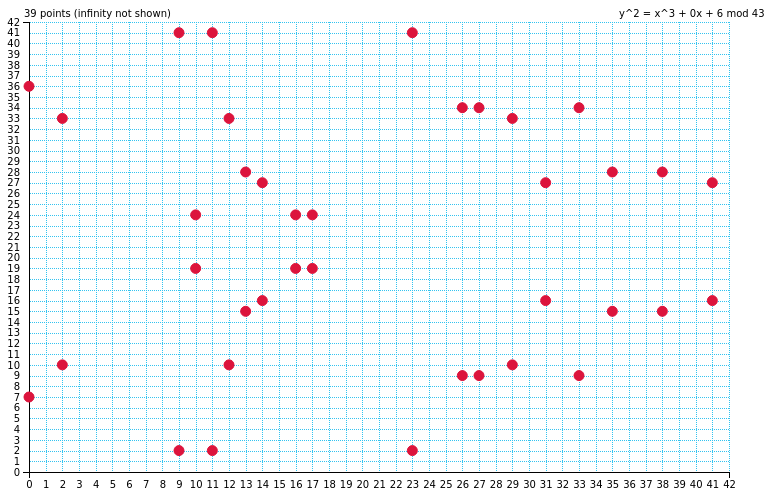
\includegraphics[scale=0.6]{figures/bls6-6.png}
As we can see our curve is somewhat nice, as it does not contain self inverse points that is points with $y=0$. It follows that the addition law can be optimized, since the branch for those cases can be eliminated. 

Note: Is there a way to printe the entire addition table from https://graui.de/code/elliptic2/ here? Would be nice to have but is a bit large.

Since the order of BLS6-6 is $39= 3\cdot 13$, we know that it has a "large" subgroup of order $13$ and small subgroup of order $3$. We can use XXX to find those groups. We have $BLS6-6(3)=\{\mathcal{O},(0,7),(0,36)\}$.

In addition we have the generator $g_{BLS6}:=(13,15)$ that generates
\begin{multline}
BLS6-6(13)=\\
\{(13,15) \rightarrow (33,34) \rightarrow  (38,15) \rightarrow  (35,28) \rightarrow (26,34) \rightarrow  (27,34) \rightarrow  \\ 
(27,9)  \rightarrow  (26,9) \rightarrow  (35,15) \rightarrow  (38,28) \rightarrow  (33,9) \rightarrow (13,28) \rightarrow  \mathcal{O}\}$$
\end{multline}

Computations "in the exponent": In cryptography and in particular in snarks a lot HAPPENS IN THE EXPONENT...

To use our example to explain what this means observe that from this representation, we can deduce a map from the scalar field $\F_{13}$ to $BLS6-6(13)$ with respect to our generator. WE have
$$
[\cdot]_{(13,15)}: \F_{13} \to BLS6-6(13)\;;\; x \mapsto [x](13,15)
$$

So for example we have $[1]_{(13,15)}= (13,15)$, $[7]_{(13,15)}= (27,9)$ and $[0]_{(13,15)}= \mathcal{O}$. In particular this map is a homomorphism of groups from the additive group $\F_{13}$ to $BLS6-6(13)$. This means in particular, the the additive neutral element from $\F_{13}$ is mapped to $\mathcal{O}$ and negatives are mapped to inverses. For example $[-2]_{(13,15)}= - [2]_{(13,15)}$, since
$[-2]_{(13,15)}= [11]_{(13,15)}= (33,9) = (33,-34) = -(33,34)=
- [2]_{(13,15)}$

The map also give a visualization of the ECDL problem in $BLS6-6(13)$, which is concerned with finding solutions $x\in \F_{13}$ for the equation 
$[x]_{(13,15)}= (x,y)$ for any $(x,y) \in BLS6-6(13)$. Of course ECDL is not hard in $BLS6-6(13)$, since we can deduce the solutions easily from XXX. For example the solution to $[x]_{(13,15)}= (35,15)$ is $x=9$, since $[9](13,15)=(35,15)$.

Since $[0]_{(13,15)}$ maps the group of cyclic integers modulo $13$ onto our group $BLS6-6(13)$, we can use this to write down the group law in the following way:
\begingroup
    \fontsize{5pt}{5pt}\selectfont
$$
\begin{array}{c|ccccccccccccc}
\cdot & \mathcal{O}  & (13,15) & (33,34) & (38,15) & (35,28) & (26,34) & (27,34) & (27,9) & (26,9) & (35,15) & (38,28) & (33,9) & (13,28)\\
\hline
\\
\mathcal{O} & \mathcal{O}  & (13,15) & (33,34) & (38,15) & (35,28) & (26,34) & (27,34) & (27,9) & (26,9) & (35,15) & (38,28) & (33,9) & (13,28)\\
\\
(13,15) & (13,15) & (33,34) & (38,15) & (35,28) & (26,34) & (27,34) & (27,9) & (26,9) & (35,15) & (38,28) & (33,9) & (13,28) & \mathcal{O}\\
\\
(33,34) & (33,34) & (38,15) & (35,28) & (26,34) & (27,34) & (27,9) & (26,9) & (35,15) & (38,28) & (33,9) & (13,28) & \mathcal{O} & (13,15)\\
\\
(38,15) & (38,15) & (35,28) & (26,34) & (27,34) & (27,9) & (26,9) & (35,15) & (38,28) & (33,9) & (13,28) & \mathcal{O} & (13,15) & (33,34)\\
\\
(35,28) & (35,28) & (26,34) & (27,34) & (27,9) & (26,9) & (35,15) & (38,28) & (33,9) & (13,28) & \mathcal{O} & (13,15) & (33,34) & (38,15)\\
\\
(26,34) & (26,34) & (27,34) & (27,9) & (26,9) & (35,15) & (38,28) & (33,9) & (13,28) & \mathcal{O} & (13,15) & (33,34) & (38,15) & (35,28)\\
\\
(27,34) & (27,34) & (27,9) & (26,9) & (35,15) & (38,28) & (33,9) & (13,28) & \mathcal{O} & (13,15) & (33,34) & (38,15) & (35,28) & (26,34)\\
\\
(27,9) & (27,9) & (26,9) & (35,15) & (38,28) & (33,9) & (13,28) & \mathcal{O} & (13,15) & (33,34) & (38,15) & (35,28) & (26,34) & (27,34)\\
\\
(26,9) & (26,9) & (35,15) & (38,28) & (33,9) & (13,28) & \mathcal{O} & (13,15) & (33,34) & (38,15) & (35,28) & (26,34) & (27,34) & (27,9)\\
\\
(35,15) & (35,15) & (38,28) & (33,9) & (13,28) & \mathcal{O} & (13,15) & (33,34) & (38,15) & (35,28) & (26,34) & (27,34) & (27,9) & (26,9)\\
\\
(38,28) & (38,28) & (33,9) & (13,28) & \mathcal{O} & (13,15) & (33,34) & (38,15) & (35,28) & (26,34) & (27,34) & (27,9) & (26,9) & (35,15)\\
\\
(33,9) & (33,9) & (13,28) & \mathcal{O} & (13,15) & (33,34) & (38,15) & (35,28) & (26,34) & (27,34) & (27,9) & (26,9) & (35,15) & (38,28)\\
\\
(13,28) & (13,28) & \mathcal{O} & (13,15) & (33,34) & (38,15) & (35,28) & (26,34) & (27,34) & (27,9) & (26,9) & (35,15) & (38,28) & (33,9)\\
\end{array}
$$
\endgroup


Cofactor clearing: 

Given an arbitrary point on the curve that is not in any of our two subgroups like $(2,33)$, we can project it on both subgroups $BLS6-6(3)$ and $BLS6-6(13)$ respectively, by \textit{multiplication with the cofactor}. Since $39 = 3 \cdot 13$, we have to multiply $(2,33)$ with $13$ to map it onto $BLS6-6(3)$ and we have to multiply $(2,33)$ with $3$ to map it onto $BLS6-6(13)$. Indeed we get $[13](2,33)= (0,36)$ which is an element of $BLS6-6(3)$ and $[3](2,33)= (35,15)$ which is an element of $BLS6-6(13)$

In what follows we want to compute type 2 pairings on our BLS6 curve. We therefore need to extract the subgroup $\mathbb{G}_1$ as well as $\mathbb{G}_2$ from the full $13$-torsion group. We already know from XXX that $\mathbb{G}_1$ is given by  
\begin{multline*}
\mathbb{G}_1=\{(13,15) \rightarrow (33,34) \rightarrow  (38,15) \rightarrow  (35,28) \rightarrow (26,34) \rightarrow  (27,34) \rightarrow  \\ 
(27,9)  \rightarrow  (26,9) \rightarrow  (35,15) \rightarrow  (38,28) \rightarrow  (33,9) \rightarrow (13,28) \rightarrow  \mathcal{O}\}$$
\end{multline*}

In type 2 pairings, the group $\mathbb{G}_2$ is defined by those elements $P$ of the full $13$-torsion group, that are mapped to $43\cdot P$ under the Frobenius endomorphism XXX. Since $BLS6/\F_{13^6}$ contains $6321251664$ elements, we can not simply loop through all elements, to find the full $13$-torsion group and extract all elements from $\mathbb{G}_2$. However we can derive the full $13$-torsion as the set of all $13$-division points and then extract $G_2$ from this
\begin{sagecommandline}
sage: F43 = GF(43)
sage: F43t.<t> = F43[]
sage: F43_6.<v> = GF(43^6, name='v', modulus=t^6+6) # t^6+6 irreducible
sage: BLS6 = EllipticCurve (F43_6,[0 ,6])
sage: INF = BLS6(0) # point at infinity
sage: for P in INF.division_points(13): # PI(P) == [q]P
....:     if P.order() == 13: # exclude point at infinity
....:         PiP = BLS6([a.frobenius() for a in P])
....:         qP = 43*P
....:         if PiP == qP:
....:             print(P.xy())
\end{sagecommandline}

Choose $g_2=(7v^2, 16v^3)$ as generator of $\mathbb{G}_2$, we get
\begin{multline*}
\mathbb{G}_2=\{
(7v^2, 16v^3) \to
(10v^2, 28v^3)\to
(42v^2, 16v^3)\to
(37v^2, 27v^3)\to\\
(16v^2, 28v^3)\to
(17v^2, 28v^3)\to
(17v^2, 15v^3)\to
(16v^2, 15v^3)\to\\
(37v^2, 16v^3)\to
(42v^2, 27v^3)\to
(10v^2, 15v^3)\to
(7v^2, 27v^3)\to
\mathcal{O}\}
\end{multline*}
e.g. $[3]g_2= (42v^2, 16v^3)$.

Having those groups we can do pairings. We choose the Weil pairing and invoke sagemath. For example the Weil pairing between our two generators is
$$
e(g_1,g_2)= 5v^5 + 16v^4 + 16v^3 + 15v^2 + 3v + 41
$$

\begin{sagecommandline}
sage: g1 = BLS6([13,15])
sage: g2 = BLS6([7*v^2, 16*v^3])
sage: g1.weil_pairing(g2,13)
\end{sagecommandline}

As we have seen, $\mathbb{G}_2$ needs quite a bit more storage space then $\mathbb{G}_1$, since elements in $\mathbb{G}_2$ are pairs of polynomials of degree $<6$ with coefficients in $\F_{43}$, while elements from $\mathbb{G}_1$ are just pairs of elements from $\F_{43}$. 

As we know from XXX it is possible to reduce the space needed to store $\mathbb{G}_2$ by using the concept of a twist. In our case $BLS6$ has embedding degree $6$ and the curve parameter $a$ in $y^2 = x^3 +ax + b$ is zero. We therefore know from XXX, that BLS6 has three different twist: A quadratic twist, a cubic twist and a sextic twist. We want to compute all of these twist:

The quadratic twisted BLS6-6 curve: Consider our BLS6-6 curve $BLS6-6/\F_{43^6}$. A quadratic twist is then another curve $BLS6-6_{2-twist}$ over $\F_{43^3}$ isomorphic to the original curve. We use XXX. The task is to find an $\omega\in \F_{43^6}$, such that $\omega^2 \in \F_{43^3}$. 
We choose $\omega = x^4 + 7x^3 + 9x^2 + 11x + 8$. Then we interpret $\delta = \omega^2 = 27x^2 + 17x + 35$ as an element from $\F_{43^3}$. So our twisted curve is
$y^2 = x^3+a\delta^2 x+b \delta^3 = x^3+6\cdot(27t^2+17t+35)$
so we get
$$
BLS6-6_{2-twist}/\F_{43^3}: y^2 = x^3+(10t^2+14t+15)
$$
\subsubsection{Baby JubJub}
% As we talk about R1CS already may write elliptic curves chapter after circuits/r1cs?
To give an understanding what the Baby-JubJub curve is, we want to parallel its development here to find a Baby-Jubjub like curve for pen and paper.

As with the original large Baby-JubJub curve we apply the method from
%https://www.hjp.at/doc/rfc/rfc7748.html#page_19 (Appendinx A)
to define a pen\& paper Baby-JubJub-like curve over the scalar field of the "large" BLS6 prime order subgroup, which is $\F_{13}$. 

Since $\Zmod{13}{4}=1$ we would go with A.1. As we will only find a few curves, we will tweak the algorithm and run
\begin{sagecommandline}
sage: F13 = GF(13) 
sage: for A in xrange(3, 13):
....:     if (A-2) % 4 != 0:
....:         continue
....:     try:
....:         E = EllipticCurve(F13, [0, A, 0, 1, 0]) # Montgomery form
....:         E
....:         E.order()
....:     except:               
....:         continue      
\end{sagecommandline}
So we get two curves in Montgomery form $y^2 = x^3 + 6*x^2 + x$ which has order $8$ and  $y^2 = x^3 + 10*x^2 + x$, which has order $16$. We could transform one of them into an Edwards curve, however   

So to find our Edwards curve, we will do exhaustive search rather 
\begin{sagecommandline}
sage: for d in F13:          
....:     j= ZZ(0)          
....:     for x in F13:
....:         for y in F13:                        
....:             if x^2+y^2 == 1+d*x^2*y^2:                           
....:                 j=j+1        
....:     print('d=',d)                
....:     print('order=',j)     
\end{sagecommandline}
and get $x^2+y^2= 1+7\cdot x^2y^2$ which has $20$ points. The associated Montgomery curve is then using XXX given by $8y^2 = x^3 + 6\cdot x^2 + x$.

So we define our Baby-JubJub Edwards curve to be
$$
EdBJJ/\F_{13}: x^2+y^2= 1+7\cdot x^2y^2
$$
with associated Montgomery form to be
$$
MBJJ/\F_{13}:8y^2 = x^3 + 6\cdot x^2 + x
$$
As $20=2\cdot 2\cdot 5$, we have a "large" prime order subgroup of order $5$ and a cofactor $4$. The group of rational points is
\begin{sagecommandline}
sage: for x in F13:                                   
....:     for y in F13:                                                                                
....:         if x^2+y^2 == F13(1)+F13(7)*x^2*y^2:                                                     
....:             print(x,y)
\end{sagecommandline}

$$
(0, 1),
(0, 12),
(1, 0),
(2, 4),
(2, 9),
(4, 2),
(4, 11),
(5, 6),
(5, 7),
(6, 5),
(6, 8),
(7, 5),
(7, 8),
(8, 6),
(8, 7),
(9, 2),
(9, 11),
(11, 4),
(11, 9),
(12, 0)
$$
with neutral element $(0,12)$

As expected we have a prime order subgroup of size $5$, which can be generated by $(11,9)$. We get $\{(11,9)\to (6,8)\to (7,8) \to (2,9) \to (0,1))\}$.

% rewrite into something nice
\begin{sagecommandline}
sage: def Edwards_add((x1,y1),(x2,y2),d):
....:     x3 = F13((F13(x1)*F13(y2)+F13(y1)*F13(x2))/((F13(1)+F13(d)*F13(x1)*F13
....: (x2)*F13(y1)*F13(y2))))
....:     y3 = F13((F13(y1)*F13(y2)-F13(x1)*F13(x2))/((F13(1)-F13(d)*F13(x1)*F13
....: (x2)*F13(y1)*F13(y2))))
....:     return (x3,y3)
\end{sagecommandline}

\paragraph{Hashing to the pairing groups}
We give various constructions to hash into $\mathbb{G}_1$ and $\mathbb{G}_2$. 

We start with hashing to the scalar field... TO APPEAR

Non of these techniques work for hashing into $\mathbb{G}_2$. We therefore implement Pederson's Hash for BLS6. 

We start with $\mathbb{G}_1$. Our goal is to define an $12$-bit bounded hash function
$$
H_{1}: \{0,1\}^{12} \to \mathbb{G}_1 
$$
Since $12= 3\cdot 4$ we "randomly" select $4$ uniformly distributed generators $\{(38, 15), (35,28), (27, 34), (38, 28)\}$ from $\mathbb{G}_1$ and use the pseudo-random function from XXX. 
For every genrator we therefore have to choose a set of $4$ randomly generated invertible elements from $\F_{13}$. We choose
$$
\begin{array}{lcl}
(38,15) &:& \{2,7,5,9\}\\
(35,28) &:& \{11,4,7,7\}\\
(27,34) &:& \{5,3,7,12\}\\
(38,28) &:& \{6,5,1,8\}
\end{array}
$$
So our hash function is computed like this:
\begin{multline*}
H_1(x_{11},x_1,\ldots, x_{0})=
[2\cdot 7^{x_{11}}\cdot 5^{x_{10}}\cdot 9^{x_9}](38,15)+
[11\cdot 4^{x_8}\cdot 7^{x_7}\cdot 7^{x_6}](35,28)+\\
[5\cdot 3^{x_5}\cdot 7^{x_4}\cdot 12^{x_3}](27,34) +
[6\cdot 5^{x_2}\cdot 1^{x_{1}}\cdot 8^{x_{0}}](38,28)
\end{multline*}
Note that $a^x=1$ whe $x=0$ and hence those terms can be omitted in the computation. 
In particular the hash of the $12$-bit zero string is given by 
\begin{multline*}WRONG-ORDERING-REDO
H_1(0)= [2](38,15)+[11](35,28)+[5](27,34)+[6](38,28)= \\
(27,34)+(26,34)+(35,28)+(26,9)= (33,9) + (13,28) = (38,28)
\end{multline*}
The hash of $011010101100$ is given by 
\begin{multline*}
H_1(011010101100)=WRONG-ORDERING-REDO\\
[2\cdot 7^{0}\cdot 5^{1}\cdot 9^{1}](38,15)+
[11\cdot 4^{0}\cdot 7^{1}\cdot 7^{0}](35,28)+
[5\cdot 3^{1}\cdot 7^{0}\cdot 12^{1}](27,34) +
[6\cdot 5^{1}\cdot 1^{0}\cdot 8^{0}](38,28)=\\
[2\cdot 5\cdot 9](38,15)+
[11\cdot 7](35,28)+
[5\cdot 3\cdot 12](27,34) +
[6\cdot 5](38,28)=\\
[12](38,15)+
[12](35,28)+
[11](27,34) +
[4](38,28)=\\ 
TO_APPEAR
\end{multline*}
We can use the same technique to define a $12$-bit bounded hash function in $\mathbb{G}_2$:  
$$
H_{2}: \{0,1\}^{12} \to \mathbb{G}_2 
$$
Again we "randomly" select $4$ uniformly distributed generators $\{(7v^2 , 16v^3 ), (42v^2 , 16v^3 ), (17v^2 , 15v^3 ), (10v^2 , 15v^3 )\}$ from $\mathbb{G}_2$ and use the pseudo-random function from XXX. For every genrator we therefore have to choose a set of $4$ randomly generated invertible elements from $\F_{13}$. We choose
$$
\begin{array}{lcl}
(7v^2 , 16v^3 ) &:& \{8,4,5,7\}\\
(42v^2 , 16v^3 ) &:& \{12,1,3,8\}\\
(17v^2 , 15v^3 ) &:& \{2,3,9,11\}\\
(10v^2 , 15v^3 ) &:& \{3,6,9,10\}
\end{array}
$$
So our hash function is computed like this:
\begin{multline*}
H_1(x_{11},x_{10},\ldots, x_{0})=
[8\cdot 4^{x_{11}}\cdot 5^{x_{10}}\cdot 7^{x_9}](7v^2 , 16v^3)+
[12\cdot 1^{x_8}\cdot 3^{x_7}\cdot 8^{x_6}](42v^2 , 16v^3 )+\\
[2\cdot 3^{x_5}\cdot 9^{x_4}\cdot 11^{x_3}](17v^2 , 15v^3 ) +
[3\cdot 6^{x_2}\cdot 9^{x_{1}}\cdot 10^{x_{0}}](10v^2 , 15v^3 )
\end{multline*}
We extend this to a hash function that maps unbounded bitstring to $\mathbb{G}_2$ by precomposing with an actual haah function like $MD5$ and feet the first 12 bits of its outcome into our previously defined hash function. 
$$
TinyMD5_{\mathbb{G}_2}: \{0,1\}^* \to \mathbb{G}_2
$$
with $TinyMD5_{\mathbb{G}_2}(s)= H_2(MD5(s)_0,\ldots MD5(s)_{11})$. For example, since 
$MD5("")= 0xd41d8cd98f00b204e9800998ecf8427e$ and the binary representation of the hexadecimal number $0x27e$ is $001001111110$ we compute $TinyMD5_{\mathbb{G}_2}$ of the empty string as
$TinyMD5_{\mathbb{G}_2}("")= H_2(MD5(s)_{11},\ldots MD5(s)_{0}) = H2(001001111110)=$

\subsubsection{Baby-JubJub-2}
To give an understanding what the Baby-JubJub curve is, we want to parallel its development here to find a Baby-Jubjub like curve for pen and paper.

The original Baby-JubJub is a twisted Edwards curve over $\F_{?}$ with $a=-1$ and $d=?.$

As with the original large Baby-JubJub curve we apply the method from
%https://www.hjp.at/doc/rfc/rfc7748.html#page_19 (Appendinx A)
to define a pen\& paper Baby-JubJub-like curve over the scalar field of the "large" BLS6 prime order subgroup, which is $\F_{13}$. 

Since $\Zmod{13}{4}=1$ we would go with A.1. As we will only find a few curves, we will tweak the algorithm and run
\begin{sagecommandline}
sage: F13 = GF(13) 
sage: for A in xrange(3, 13):
....:     if (A-2) % 4 != 0:
....:         continue
....:     try:
....:         E = EllipticCurve(F13, [0, A, 0, 1, 0]) # Montgomery form
....:         E
....:         E.order()
....:     except:               
....:         continue      
\end{sagecommandline}
So we get two curves in Montgomery form $y^2 = x^3 + 6*x^2 + x$ which has order $8$ and  $y^2 = x^3 + 10*x^2 + x$, which has order $16$. We could transform one of them into an Edwards curve, however   

So to find our Edwards curve, we will do exhaustive search rather 
\begin{sagecommandline}
sage: j = ZZ(0)
sage: for a in F13:
....:     for d in F13:
....:         j = 0
....:         for x in F13:
....:             for y in F13:
....:                 if a*x^2 + y^2 == 1+d*x^2*y^2:
....:                     j=j+1
....:         print('curve: a=',a,'d=',d,'order:',j)     
\end{sagecommandline}
We want to choose a curve that has a large prime order subgroup and a small cofactor. So we go
with $2x^2+y^2= 1+3\cdot x^2y^2$ which has order $14$. 


The associated Montgomery curve is then using XXX given by $9y^2 = x^3 +2x^2 + x$.

So we define our Baby-JubJub Edwards curve to be
$$
EdBJJ/\F_{13}: 2x^2+y^2= 1+3\cdot x^2y^2
$$
with associated Montgomery form to be
$$
MBJJ/\F_{13}:9y^2 = x^3 + 2x^2 + x
$$
As $14=2\cdot 7$, we have a "large" prime order subgroup of order $7$ and a cofactor $2$. The group of rational points is
\begin{sagecommandline}
sage: for x in F13:                                   
....:     for y in F13:                                                                                
....:         if F13(2)*x^2+y^2 == F13(1)+F13(11)*x^2*y^2:                                                     
....:             print(x,y)
\end{sagecommandline}

$$
(0, 1),
(0, 12),
(2, 4),
(2, 9),
(4, 5),
(4, 8),
(5, 2),
(5, 11),
(8, 2),
(8, 11),
(9, 5),
(9, 8),
(11, 4),
(11, 9)
$$
with neutral element $(0,1)$

As expected we have a prime order subgroup of size $5$, which can be generated by $(11,9)$. We get $\{(11,9)\to (6,8)\to (7,8) \to (2,9) \to (0,1))\}$.

% rewrite into something nice
\begin{sagecommandline}
sage: def Edwards_add((x1,y1),(x2,y2),a,d):
....:     x3 = F13((F13(x1)*F13(y2)+F13(y1)*F13(x2))/((F13(1)+F13(d)*F13(x1)*F13(x2)*F13(y1)*F13(y2))))
....:     y3 = F13((F13(y1)*F13(y2)-F13(a)*F13(x1)*F13(x2))/((F13(1)-F13(d)*F13(x1)*F13(x2)*F13(y1)*F13(y2))))
....:     return (x3,y3)
\end{sagecommandline}




\subsection{MNT4 MNT6 Cycles}
% https://eprint.iacr.org/2006/372.pdf theorem 5.2
\begin{theorem}
Let $q$ be a prime and $E/\F_q$ be an ordinary elliptic curve such that $r= |E(Fq)|$ is a prime greater than $3$.  
\begin{itemize}
\item $E$ has embedding  degree $k= 4$ if and only if there  exists $x\in \mathbb{Z}$ such  that $t=-x$ or $t=x+1$, and $q=x^2+x+1$.\item $E$ has  embedding  degree $k= 6$ if and only if there  exists $x\in \Z$ such that $t= 1\pm 2x$ and $q=4x^2+1$.
\item There is an elliptic curve $E/\F_q$ with embedding degree $6$, discriminant $D$, and $|E(Fq)| = r$ if and only if there is an elliptic curve $E'/\F_r$ with embedding degree $4$, discriminant $D$, and $|E'(\F_r)| =q$.
\end{itemize}
\end{theorem}

We can use this theorem to find an MNT6-MNT4 cycle over very small prime fields with characteristics $>3$: 
\paragraph{MNT4}
For our MNT4 curve, we can choose $x=2$. Then $q=7$ and if we choose $t= x+1 $ then $r = q + 1 - t = 7 + 1 -3 = 5$. Therefore our MNT4 curve is a curve $y^2=x^3+ax+b$ defined over $\F_7$ that consists of $5$ points. 

To construct the actual curve we could use the complex multiplication method again, but since the parameters $a$ and $b$ are from $\F_7$ there are only $48$ possibilities so we simply loop through all possible $a$'s and $b$'s and count the curve points until we find a curve that has $5$ rational points. We get
$$
y^2 = x^3 + 4x + 1
$$
defined over $\F_7$, with scalar field $\F_5$. Since $7= 2^2+2+1$, we know from theorem XXX, that this curve has embedding degree $4$ and hence qualifies as a pen\&{}paper pairing friendly elliptic curve. Since the curve's order is a prime and therefore has no non trivial factors, it has no non trivial subgroups. The curve has the following set of elements
$$MNT4=\{(0,1)\to (0,6)\to (4,2)\to (4,5) \to \mathcal{O}\}$$ 
\begin{sagecommandline}
sage: F7 = GF(7)
sage: MNT4 = EllipticCurve (F7,[4 ,1])
sage: [P.xy() for P in MNT4.points() if P.order() > 1]
\end{sagecommandline}
The multiplication table is
\begingroup
    \fontsize{10pt}{10pt}\selectfont
$$
\begin{array}{c|ccccc}
\cdot & \mathcal{O} & (0,1) & (4,5) & (4,2) & (0,6)\\
\hline
\\
\mathcal{O} & \mathcal{O} & (0,1) & (4,5) & (4,2) & (0,6)\\
\\
(0,1) & (0,1) & (4,5) & (4,2) & (0,6) & \mathcal{O}\\
\\
(4,5) & (4,5) & (4,2) & (0,6) & \mathcal{O} & (0,1)\\
\\
(4,2) & (4,2) & (0,6) & \mathcal{O} & (0,1) & (4,5)\\
\\
(0,6) & (0,6) & \mathcal{O} & (0,1) & (4,5) & (4,2)\\
\end{array}
$$
\endgroup
In what follows we choose our generator to be $g_{MNT4}=(0,1)$.

In what follows we want to compute type 2 pairings on our MNT4 curve. We therefore need to extract the subgroup $\mathbb{G}_1$ as well as $\mathbb{G}_2$ from the full $5$-torsion group. Since the order of MNT4 is a prime number, we already know from XXX that $\mathbb{G}_1$ is given by  
$$\mathbb{G}_1=\{(0,1)\to (0,6)\to (4,2)\to (4,5) \to \mathcal{O}\}$$ 

In type 2 pairings, the group $\mathbb{G}_2$ is defined by those elements $P$ of the full $5$-torsion group, that are mapped to $7\cdot P$ under the Frobenius endomorphism XXX. Since $MNT4/\F_{7^4}$ only contains $2475$ elements, we can  loop through all elements, to find the full $5$-torsion group and extract all elements from $\mathbb{G}_2$:
\begin{sagecommandline}
sage: F7t.<t> = F7[]
sage: F7_4.<u> = GF(7^4, name='u', modulus=t^4+t+1) # embedding degree is 4
sage: MNT4 = EllipticCurve (F7_4,[4 ,1])
sage: INF = MNT4(0) # point at infinity
sage: for P in INF.division_points(5): # PI(P) == [q]P
....:     if P.order() == 5: # exclude point at infinity
....:         PiP = MNT4([a.frobenius() for a in P])
....:         qP = 7*P
....:         if PiP == qP:
....:             print(P.xy())
\end{sagecommandline}

Choose $g_2=(2u^3 + 5u^2 + 4u + 2, 2u^3 + 3u + 5)$ as generator of $\mathbb{G}_2$, we get
\begin{multline*}
\mathbb{G}_2=\{ 
(2u^3 + 5u^2 + 4u + 2, 2u^3 + 3u + 5) \to
(5u^3 + 2u^2 + 3u + 6, 2u^2 + 3u) \to \\
(5u^3 + 2u^2 + 3u + 6, 5u^2 + 4u) \to
(2u^3 + 5u^2 + 4u + 2, 5u^3 + 4u + 2)\to
\mathcal{O}\}
\end{multline*}
e.g. $[3]g_2= (5u^3 + 2u^2 + 3u + 6, 5u^2 + 4u)$.

Having those groups we can do pairings. We choose the Weil pairing and invoke sagemath. For example the Weil pairing between our two generators is
$$
e(g_1,g_2)= 5u^3 + 2u^2 + 6u
$$
\begin{sagecommandline}
sage: g1 = MNT4([0,1])
sage: g2 = MNT4(2*u^3 + 5*u^2 + 4*u + 2, 2*u^3 + 3*u + 5)
sage: g1.weil_pairing(g2,5)
\end{sagecommandline}
The full pairing table can the be written as
\begingroup
    \fontsize{10pt}{10pt}\selectfont
    
% generate the table entries as:
% sage: for i in range(5):
% ....:     for j in range(5):
% ....:         p = (i*g1).weil_pairing((j*g2),5)
% ....:         print('e([',i,']g1,[',j,']g2=',p)         
    
    
$$
\begin{array}{c|lllll}
e(\cdot,\cdot)    & \mathcal{O} & g_1            & [2]g_1         & [3]g_1         & [4]g_1\\
\hline
\\
      \mathcal{O} & 1           & 1              & 1              & 1              & 1\\
\\
              g_2 & 1           & 5u^3+2u^2+6u   & 6u^3+5u^2+6    & 2u^3+u^2+2u+3  & u^3+6u^2+6u+4\\
\\
\left[2\right]g_2 & 1           & 6u^3+5u^2+6    & u^3+6u^2+6u+4  & 5u^3+2u^2+6u   & 2u^3+u^2+2u+3\\
\\
\left[3\right]g_2 & 1           & 2u^3+u^2+2u+3  & 5u^3+2u^2+6u   & u^3+6u^2+6u+4  & 6u^3+5u^2+6\\
\\
\left[4\right]g_2 & 1           & u^3+6u^2+6u+4  & 2u^3+u^2+2u+3  & 6u^3+5u^2+6    & 5u^3+2u^2+6u\\
\end{array}
$$
\endgroup

\paragraph{MNT6}
For our MNT6 curve, we can choose $x=1$. Then $q=5$ and if we choose $t= 1 + 2x $ then $r= q + 1 - t = 5 + 1 + 1 = 7$. Therefore our MNT6 curve is a curve $y^2=x^3+ax+b$ defined over $\F_5$ that consists of $7$ points. 

To construct the actual curve we could use the complex multiplication method again, but since the parameters $a$ and $b$ are from $\F_5$ there are only $24$ possibilities, we simply loop through all possible $a$'s and $b$'s and count the curve points until we find a curve that has $7$ rational points. We get
$$
y^2 = x^3 + 2x + 1
$$
defined over $\F_5$. Since $5= 4\cdot 1 + 1$, we know from theorem XXX, that this curve has embedding degree $6$ and hence qualifies as a pen\&{}paper pairing friendly elliptic curve. 

The curve has the following set of elements
$$MNT6=\{(1,2)\to (3,3)\to (0,1)\to (0,4)\to (3,2)\to (1,3)\to \mathcal{O}\}$$
The multiplication table is
\begingroup
    \fontsize{10pt}{10pt}\selectfont
$$
\begin{array}{c|ccccccc}
\cdot & \mathcal{O} & (1,2) & (3,3) & (0,1) & (0,4) & (3,2) & (1,3)\\
\hline
\\
\mathcal{O} & \mathcal{O} & (1,2) & (3,3) & (0,1) & (0,4) & (3,2) & (1,3)\\
\\
(1,2) & (1,2) & (3,3) & (0,1) & (0,4) & (3,2) & (1,3) & \mathcal{O}\\
\\
(3,3) & (3,3) & (0,1) & (0,4) & (3,2) & (1,3) & \mathcal{O} & (1,2)\\
\\
(0,1) & (0,1) & (0,4) & (3,2) & (1,3) & \mathcal{O} & (1,2) & (3,3)\\
\\
(0,4) & (0,4) & (3,2) & (1,3) & \mathcal{O} & (1,2) & (3,3) & (0,1)\\
\\
(3,2) & (3,2) & (1,3) & \mathcal{O} & (1,2) & (3,3) & (0,1) & (0,4)\\
\\
(1,3) & (1,3) & \mathcal{O} & (1,2) & (3,3) & (0,1) & (0,4) & (3,2)\\
\end{array}
$$
\endgroup

In what follows we choose our generator to be $g_{MNT6}=(1,2)$.

In what follows we want to compute type 2 pairings on our MNT6 curve. We therefore need to extract the subgroup $\mathbb{G}_1$ as well as $\mathbb{G}_2$ from the full $7$-torsion group. Since the order of MNT6 is a prime number, we already know from XXX that $\mathbb{G}_1$ is given by
$$\mathbb{G}_1=\{(1,2)\to (3,3)\to (0,1)\to (0,4)\to (3,2)\to (1,3)\to \mathcal{O}\}$$
In type 2 pairings, the group $\mathbb{G}_2$ is defined by those elements $P$ of the full $7$-torsion group, that are mapped to $5\cdot P$ under the Frobenius endomorphism XXX. Since $MNT6/\F_{5^6}$ contains $15680$ elements, we can still loop through all elements, to find the full $7$-torsion group and extract all elements from $\mathbb{G}_2$

\begin{sagecommandline}
sage: G.<x> = GF(5^6) # embedding degree is 6
sage: MNT6 = EllipticCurve (G,[2 ,1])
sage: INF = MNT6(0) # point at infinity
sage: for P in INF.division_points(7): # PI(P) == [q]P
....:     if P.order() == 7: # exclude point at infinity
....:         PiP = MNT6([a.frobenius() for a in P])
....:         qP = 5*P
....:         if PiP == qP:
....:             print(P.xy())
\end{sagecommandline}

\begin{multline*}
\mathbb{G}_2=\{ 
(x^3+2x^2+4x,x^5+2x^4+4x^3+3x^2+3)\to
(x^5+4x^4+2x^3+3x^2+x+2,3x^4+2x^3+x)\to\\
(4x^5+x^4+2x^3,3x^5+x^4+x^3+4x+4)\to
(4x^5+x^4+2x^3,2x^5+4x^4+4x^3+x+1) \to\\
(x^5+4x^4+2x^3+3x^2+x+2,2x^4+3x^3+4x)\to
(x^3+2x^2+4x,4x^5+3x^4+x^3+2x^2+2)\to
\mathcal{O}\}
\end{multline*}
We choose the generator $g_2 = (x^3+2x^2+4x,x^5+2x^4+4x^3+3x^2+3)$

\begin{remark}
Note however that our MNT6 curve discriminant $D=-16(4a^3 + 27 b^2)= -16(4\cdot 2^3 + 27\cdot 1^2)=-944$, while our MNT4 curve has discriminsnt XXX. Hence our example curves are not those guranteed by theorem XXX. Those curve are both given by $y^2= x^3 + 2x +1$ over $\F_5$ and $\F_7$, respectively. However as both curves have the same defining equation, we rather choose examples that are visually distinguishable by their defining equations.
\end{remark}

\subsection{Edwards curve cycles}
